% ten_year_forecast.tex
\subsection{Ten-Year Financial Forecast}

To assist in evaluating the financial viability of the product, the following graph and data illustrate predictions of sales in the first ten years of the product's life. In the first several years, the sales volume will grow as consumer recognition and demand increase. In the fifth year, rival companies will likely produce a competitive product; without any further product improvement, PICA will experience a shrinking market demand, but continue to make a profit through the end of the decade. If, however, PICA develops a new product, the long-term trend may become greater growth instead of loss. These predictions assume a per-unit cost of \$337 and a sale price of \$400.


\begin{figure}[htbp]
 \begin{center}
  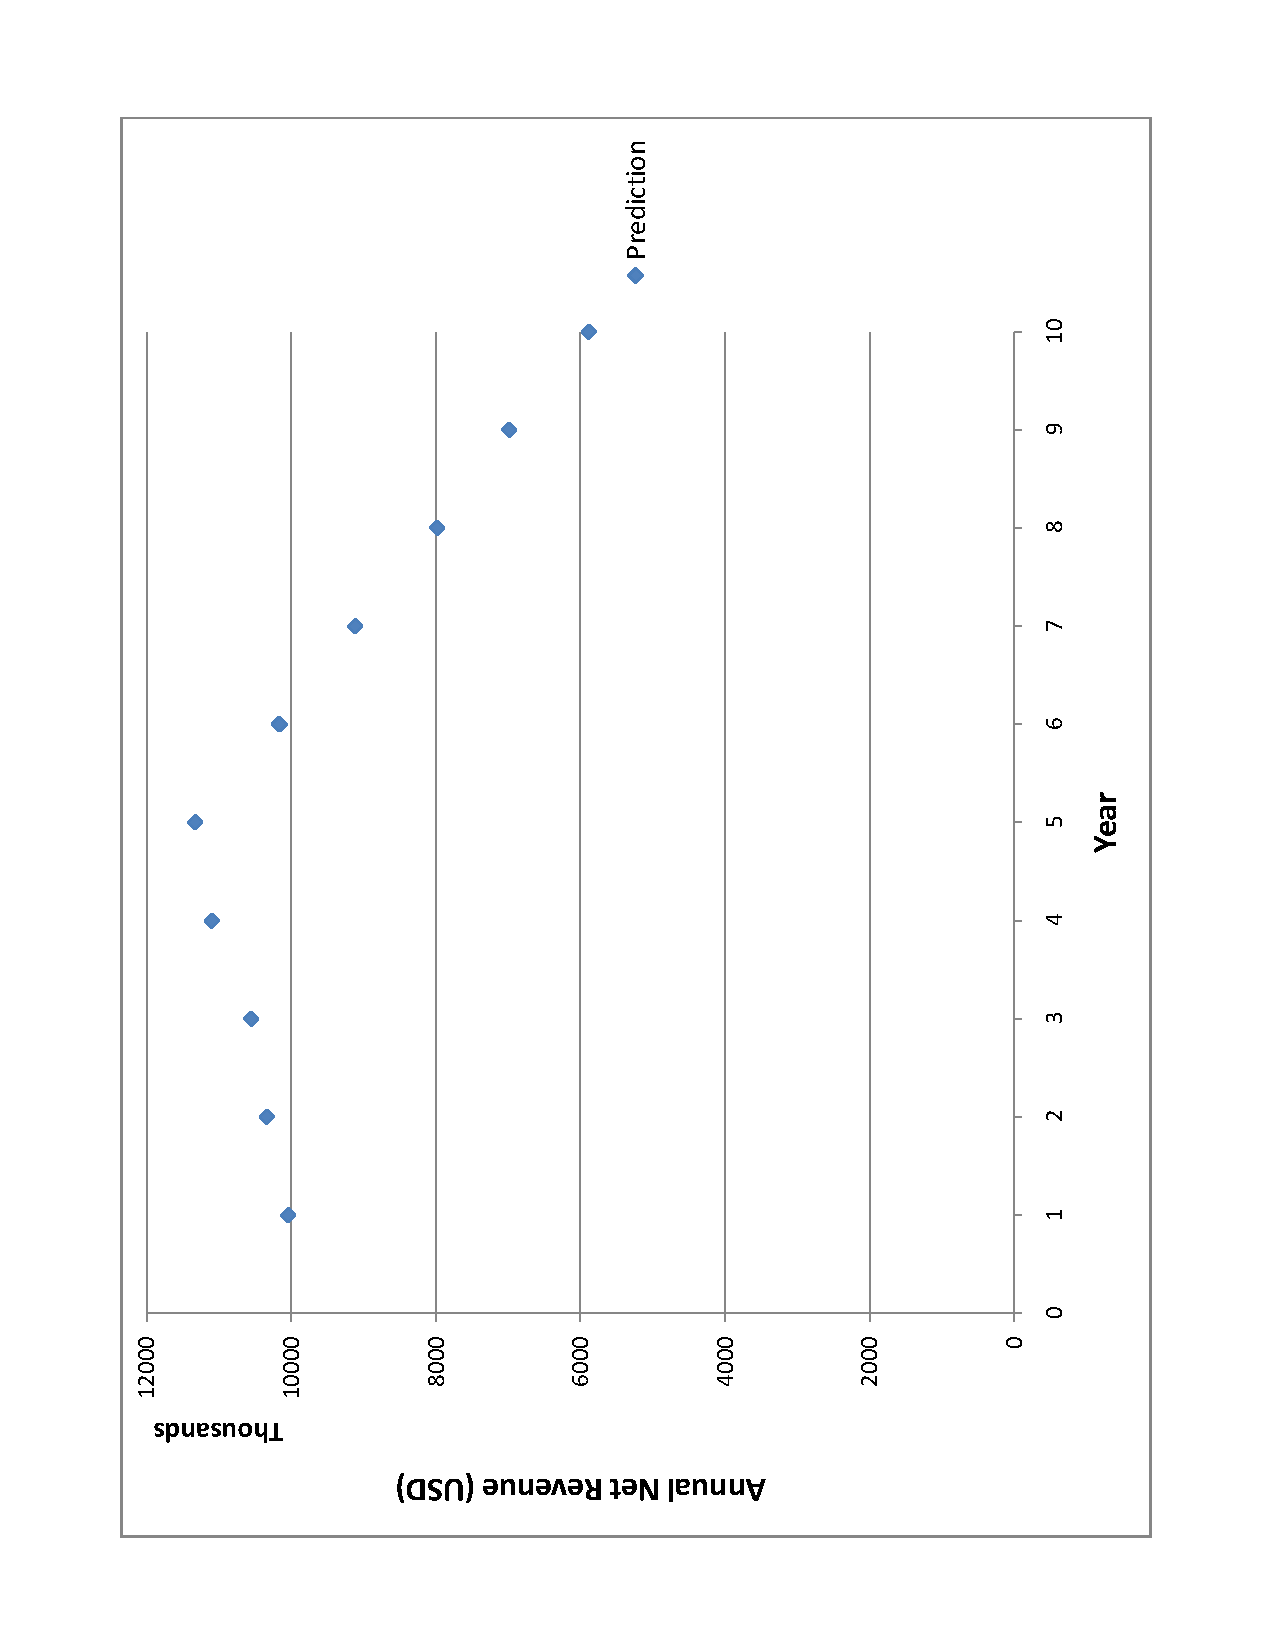
\includegraphics[angle=-90,width=5.5in]{figures/DecadeForecast}
 \end{center}
 \caption{Graph of Ten-Year Revenue Predictions}
\end{figure}

{
\small
\begin{longtable}[c]{|c|c|r|c|c|c|c|r|}
\caption{Ten-Year Financial Forecast\label{ten_year_forecast.tex}}\\
\hline
\rowcolor{lightgray}
Year & Growth & Units Sold & Parts Cost & Other Cost & Income & Balance & Running Total \\ \hline\hline
\hline
\endfirsthead

\caption[]{Continued from previous page}\\
\hline
\rowcolor{lightgray}
 Year & Growth & Units Sold & Parts Cost & Other Cost & Income & Balance & Running Total \\ \hline\hline
\hline
\endhead

\multicolumn{8}{r}{{Continued on next page}} \\
\endfoot

\endlastfoot


1 & -- & 166000 & 56000000 & 242000 & 66000000 & 10283000 & 10283000 \\
2 & +2\% & 169000 & 57000000 & 149000 & 68000000 & 10587000 & 20870000 \\
3 & +2\% & 173000 & 58000000 & 149000 & 69000000 & 10801000 & 31671000 \\
4 & +5\% & 181000 & 61000000 & 149000 & 73000000 & 11349000 & 43020000 \\
5 & +2\% & 185000 & 62000000 & 149000 & 74000000 & 11579000 & 54599000 \\
6 & -10\% & 166000 & 56000000 & 149000 & 67000000 & 10406000 & 65005000 \\
7 & -10\% & 150000 & 50000000 & 149000 & 60000000 & 9350000 & 74355000 \\
8 & -12\% & 132000 & 44000000 & 149000 & 53000000 & 8210000 & 82565000 \\
9 & -12\% & 116000 & 39000000 & 149000 & 46000000 & 7207000 & 89772000 \\
10 & -15\% & 99000 & 33000000 & 149000 & 39000000 & 6104000 & 95876000 \\
\hline
\end{longtable}
}

Table \ref{01_Final_Numbers.tex} shows the initial and recurring costs for our business. Recurring costs are further broken down into fixed and variable costs. Variable costs are shown as cost per system, independent of the volume of sales. All of the variable costs were calculated in table 6, and the initial costs were calculated in tables 4 and (hours worked; in text of document). 

{
\small
\begin{longtable}[c]{|c|c|r|}
\caption{Costs Overview\label{01_Final_Numbers.tex}}\\
\hline
\rowcolor{lightgray}
 Cost Type & Detail & Amount  \\ \hline\hline
\hline
\endfirsthead

\caption[]{Continued from previous page}\\
\hline
\rowcolor{lightgray}
 Cost Type & Detail & Amount \\ \hline\hline
\hline
\endhead

\multicolumn{3}{r}{{Continued on next page}} \\
\endfoot

\endlastfoot

\multirow{3}{*}{Initial Costs} & Facilities  & \$11,000\\\cline{2-3}
                               & Prototyping & \$82,000\\\cline{2-3}
                               & Total       & \$93,000\\\hline\hline
\multirow{4}{*}{Fixed Recurring Costs} & Marketing \& Advertising & \$120,000 \\\cline{2-3}
                                                     & Legal & \$17,000\\\cline{2-3}
                                       & Facilities & \$12,000\\\cline{2-3}
                                       & Total & \$149,000\\\hline\hline

\multirow{4}{*}{Variable Costs Per System} & Parts Cost & \$277\\\cline{2-3}
                                           & Labor      & \$44\\\cline{2-3}
                                           & Shipping   & \$16\\\cline{2-3}
                                           & Total      & \$337\\\hline

\end{longtable}
}


Table \ref{tab:02_Assembly} gives the cost of assembling each subsystem based on the number of hours needed to assemble each subsystem as estimated by the design team. Costs for wages are based on information from Professor Nielson's lecture first semester.

\input{tables/02_Assembly}

Table \ref{04_Storage.tex} calculates the cost for a storage facility where the manufactured systems can be stored until they are shipped to the customers. Floorspace needed was calculated based on the physical volume of each subsystem and how many pallets would be needed to hold a quarter of a year's supply. From this information we found the cost of a standard warehouse facility using information found at \url{www.buildingsguide.com}.

{
\small
\begin{longtable}[c]{|c|c|c|c|c|}
\caption{Storage Costs\label{04_Storage.tex}}\\
\hline
\rowcolor{lightgray}
 & Breaker Storage & E-Meter Storage & Base Station Storage & Total \\ \hline\hline
\hline
\endfirsthead

\caption[]{Continued from previous page}\\
\hline
\rowcolor{lightgray}
 & Breaker Storage & E-Meter Storage & Base Station Storage & Total \\ \hline\hline
\endhead

\multicolumn{5}{r}{{Continued on next page}} \\
\endfoot

\endlastfoot

Width ($ft$) & 0.16 & 0.5 & 1 & \\ \hline
Height ($ft$) & 0.25 & 0.67 & 0.67 & \\ \hline
Length ($ft$) & 0.33 & 0.25 & 0.33 & \\ \hline
Volume ($ft^3$) & 0.01 & 0.08 & 0.22 & \\ \hline\hline
Yearly Supply & 38,000 & 166,000 & 13,000 & \\ \hline
Quarterly Supply & 9,500 & 41,500 & 3,250 & \\ \hline\hline
Pallet Height ($ft$) & 3 & 3 & 3 & \\ \hline
Pallet Stack & 3 & 3 & 3 & \\ \hline
Total Height ($ft$) & 9 & 9 & 9 & \\ \hline\hline
Floor Area ($ft^2$) & 14 & 384 & 80 & 479 \\ \hline
Floor Length (sqare) ($ft$) & 4 & 20 & 9 & 22 \\ \hline
Cost & \$323 & \$8,832 & \$1,844 & \$11,000 \\ \hline
Per-unit Cost & \$0.03 & \$0.21 & \$0.57 & \\ \hline\hline
Yearly Supply (Peak) & 44,636 & 190,000 & 14,879 & 190,000 \\ \hline
Quarterly Supply (Peak) & 11,250 & 47,500 & 3,750 & \\ \hline\hline
Floor Area (At Peak) ($ft^2$) & 17 & 440 & 80 & 549 \\ \hline
Floor Length (Peak, Square) ($ft$) & 4 & 21 & 10 & 23 \\ \hline

\hline
\end{longtable}
}


Table \ref{05_Demand.tex} shows calculations for how many customers our business expects to have. Using the total number of electric companies and number of homes in the U.S., we determined our percentage of the market and combined this with the estimate of the total number of potential customers from the business team to find the number of systems we can expect to sell. Final numbers are given in terms of each subsystem.

{
\small
\begin{longtable}[c]{|c|c|c|r|}
\caption{Expected Demand\label{05_Demand.tex}}\\
\hline
\rowcolor{lightgray}
& Number & \multicolumn{2}{>{\columncolor[gray]{0.8}}c|}{Modified}\\ \hline\hline
\endfirsthead

\caption[]{Continued from previous page}\\
\hline
\rowcolor{lightgray}
& Number & \multicolumn{2}{>{\columncolor[gray]{0.8}}c|}{Modified}\\ \hline\hline
\endhead

\multicolumn{3}{r}{{Continued on next page}} \\
\endfoot

\endlastfoot

Customers & 6,400,000 & 1,280,000 & 1,280,000\\\hline
Percentage Interested & 0.001 & 0.0002 & 0.0002\\\hline
Customers Interested  & 64,000 & 12,800 & 13,000\\\hline\hline
Breakers/Customer & 3 & 0.6 & 0.6\\\hline
Breakers Needed & 192,000 & 38,400 & 38,000\\\hline
Base Stations Needed & 64,000 & 12,800 & 13,000 \\\hline\hline

US Power Companies & 3200 & 640 & 640\\\hline
Number Converted Homes & 8,300,000 & 1,660,000 & 1,660,000\\\hline
Number Expected Conversions & 24,900,000 & 4,980,000 & 4,980,000\\\hline
Total Homes & 130,000,000 & 260,000,000 & 260,000,000\\\hline
Average Homes/Company & 40,625 & 8,125 & 8000\\\hline\hline

Major Meter Providers & 5 & 1 & 1\\\hline
Minors Per Major & 3 & 0.6 & 0.6 \\\hline
Minor Meter Providers & 15 & 3 & 3\\\hline
Ratio Homes Provided & 3 & 0.6 & 0.6\\\hline
Effective Meter Providers & 30 & 6 & 6\\\hline\hline

PICA Homes & 830,000 & 166,000 & 166,000\\\hline
E-Meters Needed & 830,000 & 166,000 & 166,000\\\hline 

\end{longtable}
}


Table \ref{06_Cost_Per.tex} shows the costs of the subsystems as calculated in other tables and determines the cost of a full system for use in table 1. 

\input{tables/06_Cost_Per_Long}
